%%%%%%%%%%%%%%%%%%%%%%%%%%%%%%%%%%%%
% This is the template for submission to ISCA 2016
% The cls file is a modified from  'sig-alternate.cls'
%%%%%%%%%%%%%%%%%%%%%%%%%%%%%%%%%%%%

\documentclass{sig-alternate} 
\usepackage{mathptmx} % This is Times font

\newcommand{\ignore}[1]{}
\usepackage{fancyhdr}
\usepackage[normalem]{ulem}
\usepackage[hyphens]{url}
\usepackage{hyperref}
\usepackage{listings}
\usepackage[font=small,skip=0pt]{caption}


%%%%%%%%%%%---SETME-----%%%%%%%%%%%%%
\newcommand{\hpcasubmissionnumber}{NaN}
%%%%%%%%%%%%%%%%%%%%%%%%%%%%%%%%%%%%

\fancypagestyle{firstpage}{
  \fancyhf{}
\setlength{\headheight}{50pt}
\renewcommand{\headrulewidth}{0pt}
  \fancyhead[C]{} 
  \pagenumbering{arabic}
}  

\renewcommand{\lstlistingname}{Code}

\lstset{
frame=single
}

%%%%%%%%%%%---SETME-----%%%%%%%%%%%%%
\title{Extract Useful Features for Detecting Transient Faults\vspace{-2ex}} 
\author{Zhiqiang Sui, Zhefan Ye, Karthik Desingh \vspace{-5em}}
%%%%%%%%%%%%%%%%%%%%%%%%%%%%%%%%%%%%

\begin{document}
\maketitle
\thispagestyle{firstpage}
\pagestyle{plain}

%\begin{abstract}

%\end{abstract}



\section{Introduction}
This technical report presents a general pipeline to analyse the features that can be used to predict transients faults during execution of a program. Transient faults are also known as soft errors or single event upsets. These faults are caused by either alpha particles stemming from radioactive decay, or neutrons that are present in the atmosphere. These external particles add or remove charge causing electron or hole pairs absorbed by source or drain diffusion process. This fault happens for a very short period of time and hence can be masked at various stages due to various aspects. Few of the masking factors are a) logic masking b) timing masking, c) electrical masking, d) microarchitectural masking and e) software masking. Due to the presence of so many masking levels the transient faults are 80\% of the time masked. However, there are 20\% chance that a fault can show up as a fault (segmentation) in the execution of an application or given an incorrect output.

This project is motivated to find these unmasked transient faults during the execution of a program in order to provide an ability to stop the execution if a fault as occurred, flush the pipeline and run the program from the beginning as shown in the Figure~\ref{fig:teaser}. These faults are often analysed using microarchitecture simulators. Following this practice, we utilize GemFI \cite{parasyris2014gemfi} a microarchitecture simulator extended based on Gem5 {Binkert:2011:GS:2024716.2024718} to provide a fault injection tool. Using GemFI we study the fault injection mechanism and how it affects applications. In addition to that we analyse the microarchitectural events captured by the simulator to know the status of the execution. These events can be used as a features to predict the occurance of the transient faults.

Our contribution is two-fold: 1) we implemented a general pipeline that can extract meaningful features from architectural events for any target application on GemFI simulator, 2) we provide analysis on our prediction mechanism using RandomForest algorithm along with our observations.


\section{Approach}
In this section, we present our implementation for injecting faults, as well as analysis for predicting program outcome and fault types.

\subsection{Pipeline}
Figure~\ref{fig:pipeline} shows the general pipeline of our proposed system. For any target application, it is first modified to contain at least one all to initialize fault injection. Then it is compiled in the architecture X86 or ALPHA where GemFI support with the specific libraries. In this work, we choose ALPHA as our test architecture as it is lightweight and have full supports by the fault injector. Afterwards, the generated binary should be moved to the disk image serving as the virtual disk of GemFI. The specific faults are provided by the user in a file at command line. Each line of the input file specifies the attributes of a single fault. We will talk in detail about the fault injection in Section \ref{section:FI}. 

GemFI simulator simulates the execution of the target application until a fault is to be activated. When it is time, the GemFI simulator will modify the state of the hardware e.g. flip the bit or set the value to all 0 according to the fault specification. The output of the program may differ based on whether the faults have been masked or not. These outputs will serve as the labels of our training data. GemFi simulator also generates statistics of a fixed-length microarchitecture event periodically. These raw features will serve as the feature vectors of our training data. We will talk about feature extraction in detail in Section \ref{section:FE}. 

Our feature extraction and labeling module will extracts standardized features from raw features and label them according to the result of the test program. These standardized features will then feed into Machine Learning component and ML algorithms will learn meaningful features from them. We will talk about it in Section \ref{section:ML}

\begin{figure}[t]
\begin{center}
   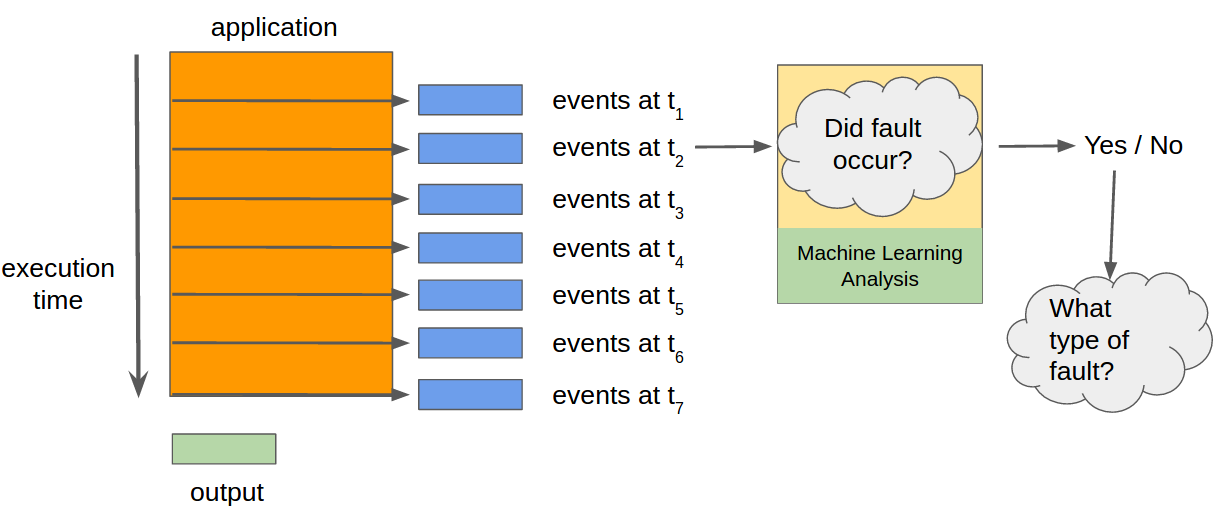
\includegraphics[width=0.95\linewidth]{./figures/teaser.png}
\end{center}
   \caption{\footnotesize Motivation to extract meaningful features}
\label{fig:teaser}
\end{figure}

\begin{figure*}[t]
\begin{center}
   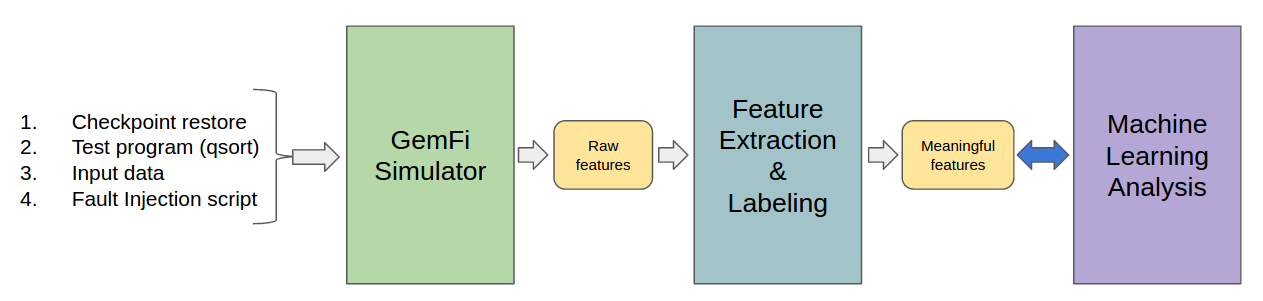
\includegraphics[width=0.95\linewidth]{./figures/pipeline.png}
\end{center}
   \caption{\footnotesize General pipeline of our work. GemFi simulator restores from the checkpoint which saves the warm up stage of the system and takes in test program, input data of the test program and the fault injection script. It then simulates the execution of the program and generates the raw features. Our feature extraction and labeling module will then extract common feature and label each feature vector for binary and multi-class classification. The machine learning algorithms learn models from the features and also output useful features.}
\label{fig:pipeline}
\end{figure*}



\subsection{Fault Injection}\label{section:FI}
The faults are provided by the user through an input file. Each line of the input file specifies the attributes of a single fault. Faults are characterized by four attributes: Location, Thread, Time and Behavior. 
\begin{itemize}
\item Location: Location specifies which microarchitectural modules the fault would be injected into, e.g. registers, the fetched instructions and PC address
\item Thread: Thread offers the flexibility for the user to selectively inject faults
\item Time: Faults are scheduled to the number of instructions already executed, or to the number of elapsed simulation ticks of the targeted thread
\item Behavior: Behavior specifies which operation the fault will corrupt the module. Flipping bits, XORing or setting all bits to 0,1 are some of the operations supported by GemFI
\end{itemize}

An example below shows the a sample input of faults. 
\begin{lstlisting}	
RegisterInjectedFault Inst:17958 Flip:16 
     Threadid:0 system.cpu1 occ:1 int 1
\end{lstlisting}

This example describes a fault that injects into the $16th$ bit of the register R1 of the CPU, when the application fetches $17958th$ instruction after the initiation of fault injection. 

In our work, we focus on four types of faults: \textit{GeneralFetchInjectedFault}, \textit{LoadStoreInjectedFault}, \textit{ExecutionInjectedFault} and \textit{OpCodeInjectedFault}. And we choose the instruction as the criteria for when to inject faults because it is easy for us to know the exact number of instructions for the test application from the output. Flipping bit is the only operation we employ for the fault as this is the most common transient fault which takes place in the real hardware. 



\subsection{Feature Extraction and Labeling}\label{section:FE}
\subsubsection{Feature Extraction}
GemFI generates a \emph{stats} file which contains the statistics for each period of microarchitecture event for different features. However, the number and type of features in each event may vary greatly because of different types of faults, different execution status and different execution results. So in order to get the fixed length of features of each event, we extract all the common features from the \emph{stats} files. 
\subsubsection{Labeling}
There are three kinds of output from the test. The first kind of faults is masked by the hardware and the result is correct. This happens a lot as the operation of flipping the bit is very likely to be masked.The second kind of faults is that the test program encounters the segmentation fault in the middle of the execution. The last kind is that the execution of the program exits normally however the output is not correct. From our trivial observation, among all the faulty execution of the program, the second kind is the one which is most commonly. We will label the first condition as 0 which is the correct output and label the latter two conditions as 1 in binary classification and 1, 2, 3, 4 corresponds to different types of fault in multi-class classification.

\subsection{Checkpoint Restoring}
We also employ checkpoint mechanism to save the simulation time of a test program. For simulating a test program, GemFI first loads the entire linux system in detailed mode and then executes the program. This loading step takes about 5 minutes and usually takes 90\% of the total simulation time. So by creating a checkpoint after the system has been loaded, we can directly simulate the test program next time by restoring this checkpoint. This saves us a lot of time when generating training data by simulating the test programs. 


\subsection{Machine Learning Method}\label{section:ML}
We use the random forest algorithm to predict program outcome and fault type. A random forest is essentially an ensemble of single decision trees \cite{breiman2001random}. It captures different characteristics of the data, with each decision tree representing a model. One particular attractive aspect of random forest is that it allows us to analyze the importance of different features according to the information gain of each feature dimensions. We can use the information gain to rank the importance of each feature and therefore determine which features can be pruned.

%\begin{figure}[t]
%\begin{center}
%   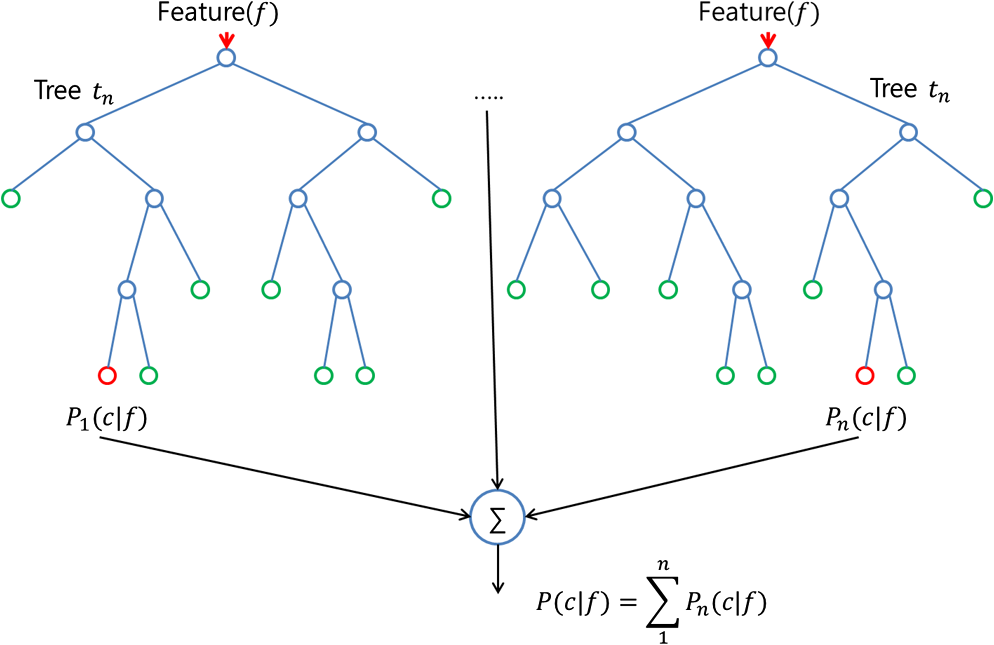
\includegraphics[width=0.95\linewidth]{./figures/rf.png}
%\end{center}
%   \caption{\footnotesize Random forests}
%\label{fig:rf}
%\end{figure}


%\begin{figure}[t]
%\begin{center}
%   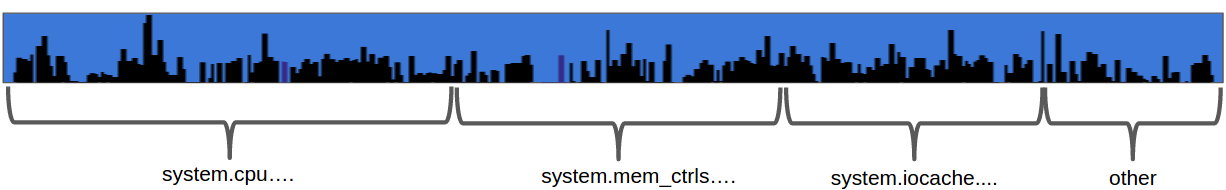
\includegraphics[width=0.95\linewidth]{./figures/feat_dist.png}
%\end{center}
%   \caption{\footnotesize Features in different components of the microachitecture.}
%   \vspace{-0.4cm}
%\label{fig:feat-dist}
%\end{figure}

%Figure~\ref{fig:feat-dist} shows features in different components of the microarchitecture.

We randomly select $60\%$ of instances for training and $40\%$ of instances for testing. Our dataset consists of $98,000$ data instance.

\section{Experiment}
In this section we describe our procedure for testing our feature extraction pipeline and machine learning methods. First we introduce our chosen test bench and metrics, followed by experimental setup.

\begin{figure}[t]
\begin{center}
   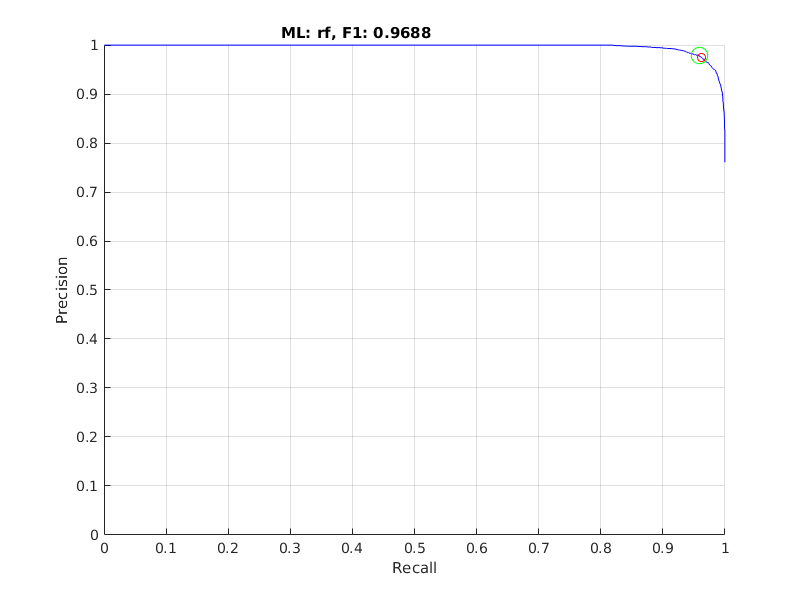
\includegraphics[width=0.8\linewidth]{./figures/siaf.png}
\end{center}
   \vspace{-0.5cm}
   \caption{Performance of the the random forest classifier using same input with all features}
   \vspace{-0.3cm}
\label{fig:siaf}
\end{figure}

\subsection{Test Bench}
We use MiBench \cite{guthaus2001mibench} as our test bench for fault injection. MiBench is a representative embedded benchmark that offers compact program sizes and versatile program characteristics. Specifically, qsort is chosen as our test program.

\subsection{Metrics}
To evaluate the performance of our machine learning method, we use precision-recall (PR) curve and $F_1$ score as our metric due to the imbalance in positive and negative samples. More precisely, we have
\begin{equation}
F_{1} = 2\cdot\frac{precision \cdot recall}{precision + recall},
\end{equation}
where $precision = \frac{tp}{tp+fp}$, $recall = \frac{tp}{tp+fn}$, $tp$ is the number true positive samples, $fp$ is number of false positive samples, and $fn$ is the number of false negative samples. $F_1$ score is the harmonic mean of precision and recall. PR curve can reflect the performance of the classifier well since it takes the number of false positives into account, which is prevalent in our testing instances. For identifying fault types, which is a multi-class classification problem, we use confusion matrix to analyse the performance of our classifier. Each column of a confusion matrix is the instances in a predicted category whereas each row is the instances in ground truth \cite{powers2011evaluation}.

\subsection{Experimental Setup}
We present four types of experiments: 1) same input data (for qsort) with all features, 2) same input data with handpicked subsets of features, 3) different input data with all meaningful features, and 4) different input data with handpicked subsets of features. With this four experiments we analyse how different inputs to the application affect the execution under fault injection, as well as how different sets of features perform in predicting the faults. This would help in coming up with an optimal strategy for feature extraction.

\section{Result}
In this section we report results of all four types of experiments. PR curves depicts the performance of the binary classifier (random forest). Confusion matrices shows how well a classifier identifies different types of faults.

\begin{figure}[t]
\begin{center}
   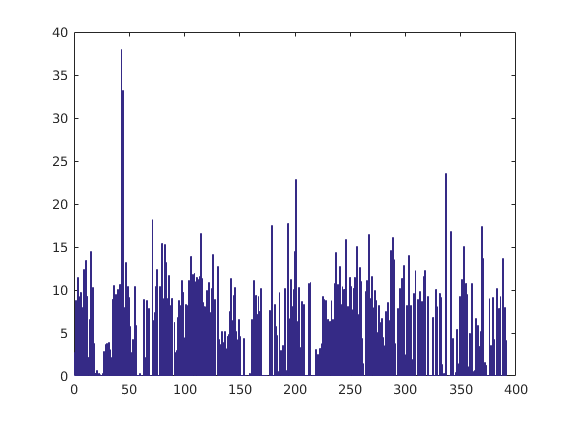
\includegraphics[width=0.8\linewidth]{./figures/feat_same.png}
\end{center}
\vspace{-0.5cm}
   \caption{Feature importance ranking of SIAF}
   \vspace{-0.3cm}
\label{fig:feat-same}
\end{figure}

\subsection{Same Input All Features (SIAF)}
Figure~\ref{fig:siaf} shows the performance of our binary classifier given all features from stats file and  when \emph{qsort} uses the same input data. In can be seen that the binary classifier performs well with an $F_1$ score of 0.9688 (max $F_1$ value: 1) along with PR curve close to the ideal classification (a curve started at $(0,1)$, reached $(1,1)$, and stopped at $(1,0)$). 

We further examine the feature importance ranking extracted from the random forest (see Figure~\ref{fig:feat-same}). The y-axis represents information gain and each bar along the x-axis represent one feature dimension. Several features in Figure~\ref{fig:feat-same} shows high discriminative power, which entails that a handful features are can predict the outcome of the program. The top-3 discriminative features are 
\begin{itemize}
\item $sim\_insts$: \\
Number of instructions simulated
\item $system.cpu.fetch.insts$: \\
Number of instructions fetch has processed
\item $system.cpu.dcache.tags.occ\_percent::cpu.data$: \\
Average percentage of cache occupancy
\end{itemize}

We further extend the capability of our classifier to predict the fault types instead of only determining program outcome. Figure~\ref{fig:siaf-multi} shows a confusion matrix of \emph{SIAF}. A perfect confusion matrix is the one with all diagonal entries in light yellow color and the non-diagonal entries in dark blue color. According to Figure~\ref{fig:siaf-multi}, our classifier can recognize correct program outcome, \emph{general fetch} fault and \emph{load/store} fault quite well. However, it doesn't perform well on \emph{execution} and \emph{opcode} fault. We suspect that this is due to the variances of those two types of faults, and we may need more training data of those two types of faults to train the classifier.

\begin{figure}[ht]
\begin{center}
   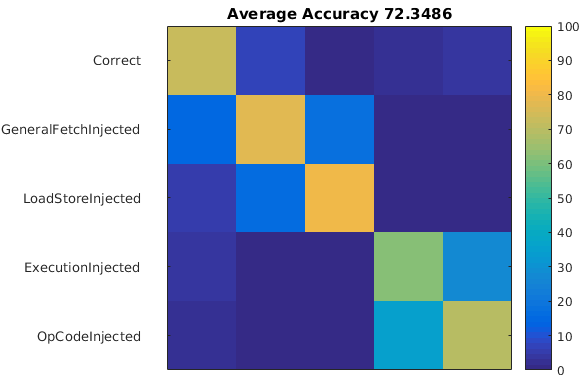
\includegraphics[width=0.8\linewidth]{./figures/siaf_multi.png}
\end{center}
\vspace{-0.3cm}
   \caption{Fault type classification using SIAF.}
\label{fig:siaf-multi}
\vspace{-0.3cm}
\end{figure}

\subsection{Same Input Different Features}
In order to examine how different sets of features may affect the performance, we further compare the PR curves of different feature sets. The broken line in Figure~\ref{fig:sidf} represents the result of using all features, which clearly outperforms all other handpicked feature. Among handpicked features, the classifier trained using $l2$ cache features performs slightly better than the rest, whereas the classifier trained using decode features performs the worst.

\begin{figure}[t]
\begin{center}
   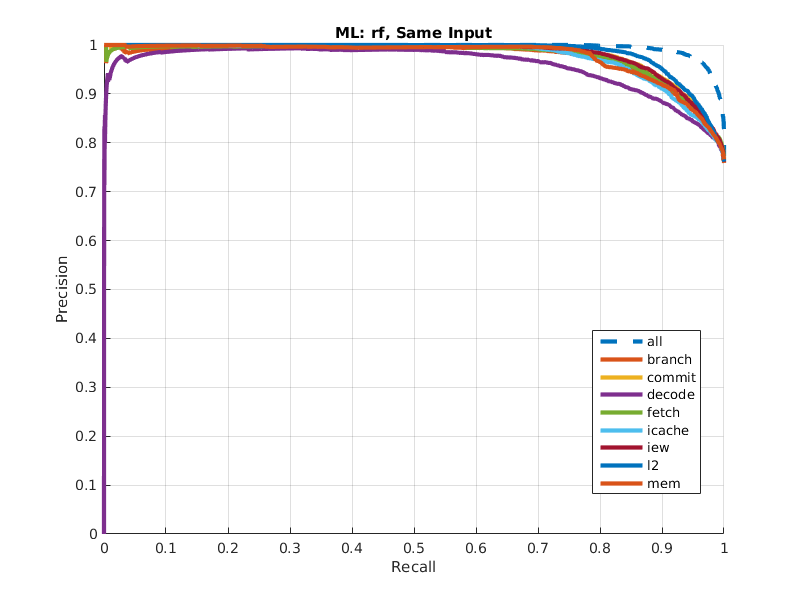
\includegraphics[width=0.95\linewidth]{./figures/sidf.png}
\end{center}
\vspace{-0.3cm}
   \caption{Comparison among classifiers trained on different sets of features using the same input data.}
\label{fig:sidf}
\vspace{-0.3cm}
\end{figure}

\subsection{Different Input}
All previous results are based on the same input data, which may not be convincing in the real-world situation. Thus, we give \emph{qsort} different input and retrain the random forest classifier.

\begin{figure}[t]
\begin{center}
   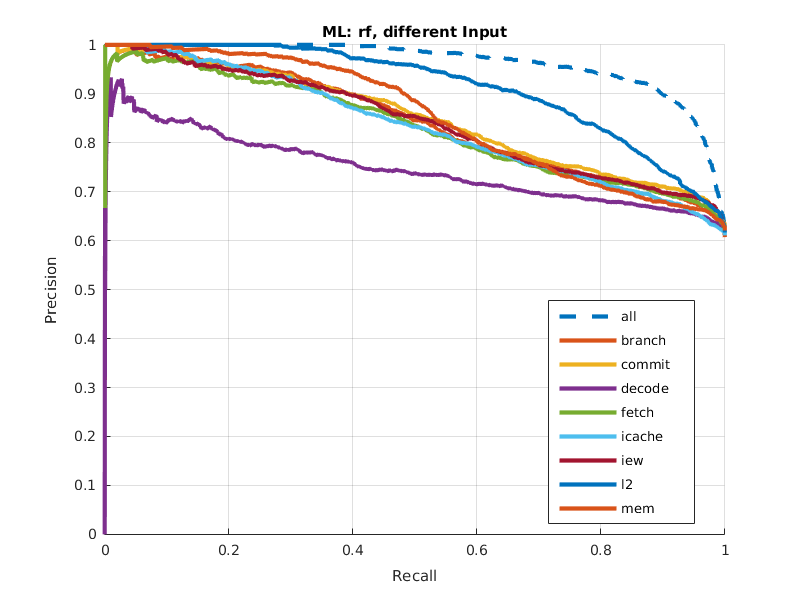
\includegraphics[width=0.8\linewidth]{./figures/didf.png}
\end{center}
\vspace{-0.3cm}
   \caption{Fault type classification using different input data.}
\label{fig:didf}
\vspace{-0.3cm}
\end{figure}

Figure~\ref{fig:didf} shows the binary classification results using different input data. The broken line represents the classifier with all features, which outperform the all other hand-picked features. This, again, demonstrates that hand-picked features may not outperform the classifier that uses all features.

\begin{figure}[t]
\begin{center}
   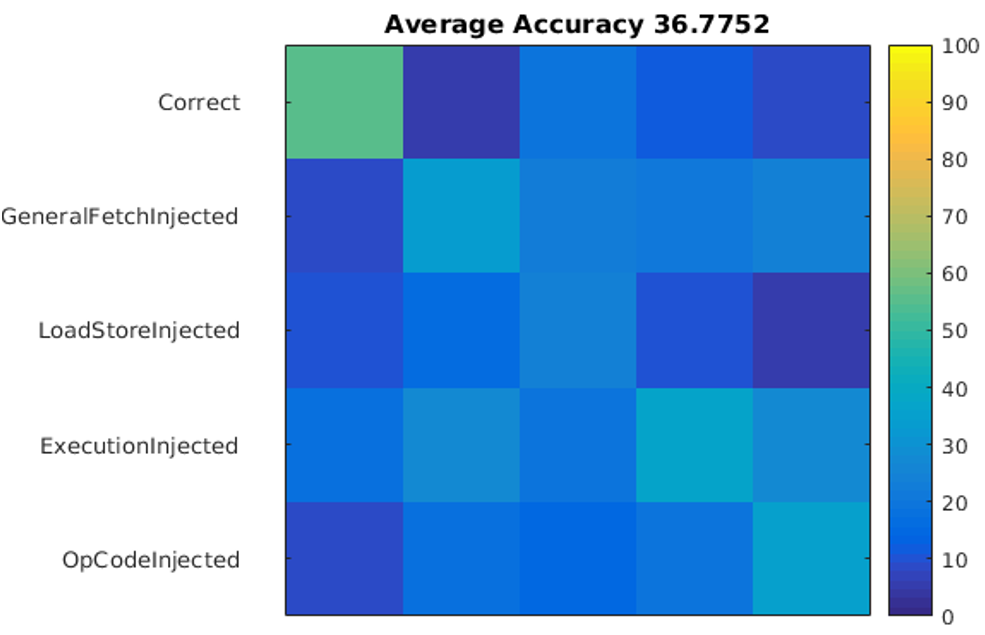
\includegraphics[width=0.8\linewidth]{./figures/diaf_multi.png}
\end{center}
\vspace{-0.3cm}
   \caption{Comparison among classifiers trained on different sets of features using the different input data.}
\label{fig:diaf-multi}
   \vspace{-0.3cm}
\end{figure}

Figure~\ref{fig:didf} shows the confusion matrix of fault prediction using different input data. Comparing to Figure \ref{fig:siaf-multi}, its performance is much worse. One reason is that different input data bring significant variance into the training data, which would require more training data to sufficiently train a classifier. Thus, given the same amount of training data, the classifier with different input data would unequivocally underperform the one with the same input data.


\section{Related Work}
There are other simulation based fault injection tools. \cite{Benso:2010:FIT:1965156}, \cite{6850649} injects faults into simulated hardware. Some tools inject faults into low-level hardware models like VERIFY\cite{614074} and MAFALDA\cite{Arlat:2002:DCM:506792.506796}. In a short time around the injection, Relyzer\cite{Hari:2012:REA:2248487.2150990} employs the meomery timing simulator and an extra microachiteural and it injects into a commerical functional full-system simulator on ISA level. There are also purely behavior-level machine simulator which injects faults directly into QEMU\cite{Bellard:2005:QFP:1247360.1247401} like F-SEFI\cite{6877352} and Qinject\cite{david2008qinject}.

\cite{4798244} uses a Machine Learning algorithm - Boosted Regression Trees to identify the correlation across workloads, execution phases and processor configurations. \cite{7757917} uses the SVM to recognize faults of the high voltage circuit breaker.
\section{Discussion and Conclusion}







%%%%%%% -- PAPER CONTENT ENDS -- %%%%%%%%

%%%%%%%%% -- BIB STYLE AND FILE -- %%%%%%%%
\bibliographystyle{ieeetr}
\bibliography{ref}
%%%%%%%%%%%%%%%%%%%%%%%%%%%%%%%%%%%%

\end{document}
